\documentclass{article}
\usepackage{amsmath, amssymb, amsthm}
\usepackage{geometry}
\usepackage{tikz}
\geometry{a4paper, margin=1in}

\title{Pointwise Continuous Mappings}
\author{Nirupam Khanal / Niv}
\date{20-Mar-2025}

\begin{document}

\maketitle

\tableofcontents 


\section{Open problem}

\begin{quote}
Consider a set of point-wise continuous mappings defined by the following transformations; which are surjective: 
\[
f_{1}, f_{2}, \dots \;:\,\|.\|\mapsto F.
\] 
\noindent \textbf{(a)} Is the function limited everywhere? \\ 
\noindent \textbf{(b)} Is the function bounded everywhere? \\ 
\end{quote}

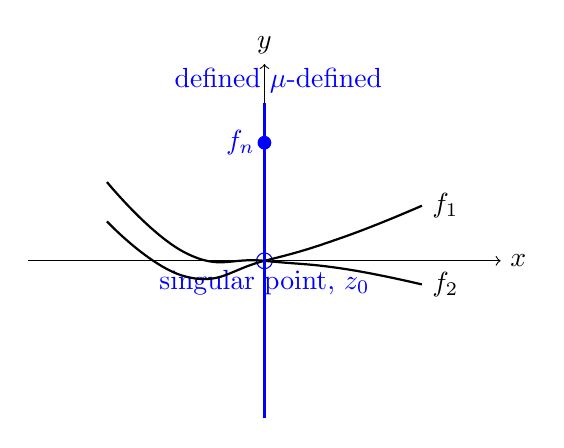
\begin{tikzpicture}[scale=1]

% Axes
\draw[->] (-3,0) -- (3,0) node[right] {$x$};
\draw[->] (0,-2) -- (0,2.5) node[above] {$y$};

% Singular point
\draw[blue, fill=white] (0,0) circle [radius=0.1] node[below] {singular point, $z_0$};

% Function curves
\draw[thick] plot [smooth, tension=0.8] coordinates {(-2,0.5) (-1,-0.2) (0,0) (1,0.3) (2,0.7)} node[right] {$f_1$};
\draw[thick] plot [smooth, tension=0.8] coordinates {(-2,1) (-1,0.1) (0,0) (1,-0.1) (2,-0.3)} node[right] {$f_2$};

% Vertical line for defined mu-DE
\draw[blue, thick] (0,-2) -- (0,2) node[above] {\quad defined $\mu$-defined};
\filldraw[blue] (0,1.5) circle [radius=0.08] node[left] {$f_n$};

\end{tikzpicture}



\end{document}